%%%%%%%%%%%%%%%%%%%%%%%%%%%%%%%%%%%%%%%%%%%%%%%%%%%%%%%%%%%%%%%%%%%%%%%%%%%%%%%%
%2345678901234567890123456789012345678901234567890123456789012345678901234567890
%        1         2         3         4         5         6         7         8
% THESIS CHAPTER

\chapter{Project management}
\label{chap:management}
\ifpdf
    \graphicspath{{Algorithms/Figures/PNG/}{EvaluationTask/Figures/PDF/}{Algorithms/Figures/}}
\else
    \graphicspath{{Algorithms/Figures/EPS/}{EvaluationTask/Figures/}}
\fi


% short summary of the chapter

A successful execution of the project required careful time management and
organisation of priorities. This section briefly outlines how this was achieved.

\section{Using GitLab} 
\label{sec:gitlab}
GitLab was the primary tool used for project management. The system offers
functionality of project tracking through Issues and Milestones. Issues were
used to define small individual tasks of the benchmark development, such as
implementing fingerprinting using constant Q transform, splitting the datasets
to train and test sets, etc. Any progress to a task was logged using comments
under the corresponding issue. GitLab milestones were used to group issues
based on the corresponding algorithm they relate to.

The git repository provided for the project on GitLab served as a main backup
and version control destination. Development of separate benchmark features was
done using \textit{feature branches} - git branches which encapsulate the
implementation process of a functionality before being merged to the master
branch after the feature is complete. Regular commits were regularly pushed to
store updated versions of the codebase. 

\begin{figure}[H]
   \centering
   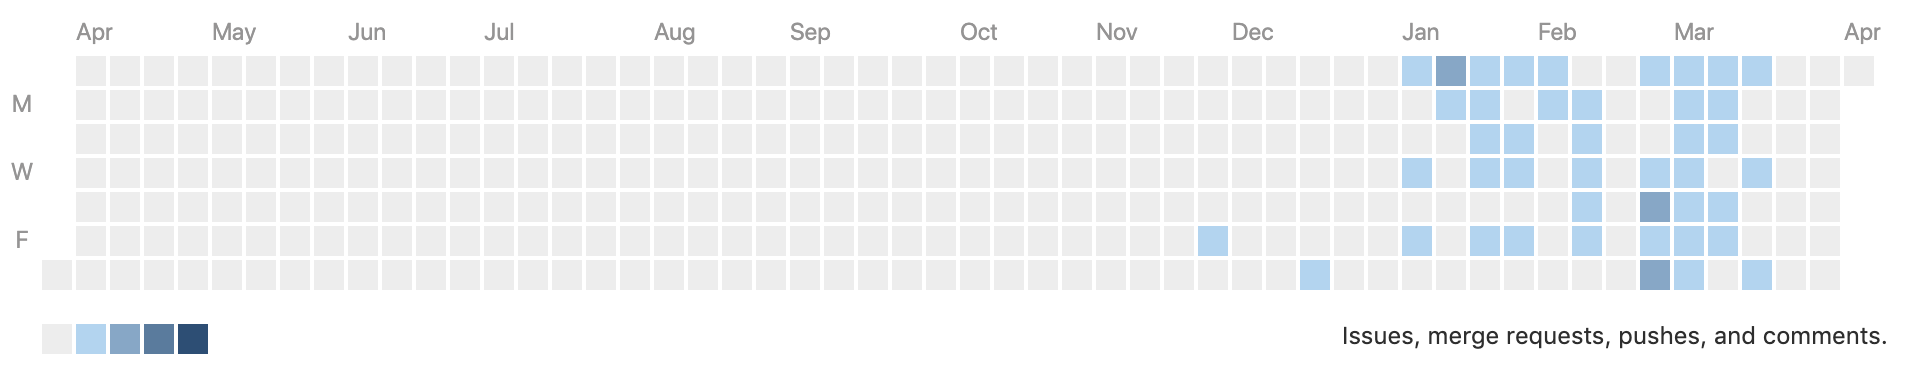
\includegraphics[width=\textwidth]{ProjectManagement/commitgraph.png}
   \captionof{figure}[GitLab project commit graph]{Overview of the frequency of commits per day of the month. Other related graphs are available in the appendix.}
   \label{fig:commitgraph}
\end{figure}

\section{Canvas logs} 
\label{sec:canvaslogs}
All Canvas logs have been submitted with information about what was done
each week. Any other logging was done through GitLab.

\section{Supervisor meetings}
\label{sec:supervisor}
Productive meetings with my supervisor took place each week. During each of them
the progress of the project was evaluated, followed by a discussion on possible
direction and targets for the upcoming week. The meetings helped me and the
project preserve its aim and focus towards the end goal.